%  !TeX  root  =  user_guide.tex

%\section{Spatial Query Plugin}\label{sec:spatial_query}
\section{Extension Requête Spatiale}\label{sec:spatial_query}

% when the revision of a section has been finalized, 
% comment out the following line:
% \updatedisclaimer

%The \toolbtntwo{spatialquery}{Spatial Query} plugin allows to make a spatial query (select features) in a target layer with reference to another layer. The functionality is based on the GEOS library and depends on the selected source feature layer. 
L'extension \toolbtntwo{spatialquery}{Requête Spatiale} permet de réaliser une requête spatiale (sélection d'entités) sur une couche cible en fonction d'une autre couche. Cette fonctionnalité est basée sur la bibliothèque GEOS, les opérations possibles dépendent de la couche source choisie.

%Possible operator are:
Les opérateurs disponibles sont :

\begin{itemize}[label=--]
%\item Crosses
\item Croise
%\item Intersects
\item Intersecte
%\item Is disjoint
\item Est disjoint
%\item Touches
\item Touche
%\item Within
\item A l'intérieur
\end{itemize}

%Polygon layers do not provide the 'Touches' and 'Crosses operator.
Les couches de polygones ne proposent pas les opérateurs 'Touche' et 'Croise'.

%\minisec{How to use the plugin}
\minisec{Comment utiliser l'extension}

%As an example we want to find regions in the Alaska dataset that contain airports. Following steps are necessary:
Nous souhaitons par exemple trouver les régions dans le jeu de données Alaska qui ont des aéroports. Les étapes suivantes sont à effectuer :

\begin{enumerate}
%  \item Start QGIS and load the vector layers regions.shp and airports.shp. 
  \item Lancez QGIS et chargez les couches vectorielles regions.shp et airports.shp.
%  \item Load the Spatial Query plugin in the Plugin Manager (see Section \ref{sec:load_core_plugin}) and click on the \toolbtntwo{spatialquery}{Spatial Query} icon which appears in the QGIS toolbar menu. The plugin dialog appears as shown   in Figure \ref{fig:spatialquerysample}.
  \item Activez l'extension Requête Spatiale dans le Gestionnaire d'extensions (voir section \ref{sec:load_core_plugin}) et cliquez sur le bouton \toolbtntwo{spatialquery}{Requête Spatiale} qui apparait dans la barre d'outils Extensions. La fenêtre de l'extension s'affiche telle que sur la figure \ref{fig:spatialquerysample}.
%  \item Select layer regions as source layer and airports as reference feature layer.
  \item Sélectionnez la couche des régions comme source et celle des aéroports comme référence.
%  \item Select 'Contains' as operator and click \button{Apply}.
  \item Sélectionnez 'A l'intérieur' comme opérateur et cliquez sur \button{Apply}.
\end{enumerate}

%Now you get a list of feature IDs from the query and you have several options.
Vous obtenez alors une liste d'identifiants des entités satisfaisant la requête. Vous avez ensuite plusieurs options :

\begin{itemize}[label=--]
%\item Click on the \toolbtntwo{selectesubsetlayer}{Create layer with list of items}
\item Cliquer sur \toolbtntwo{selectesubsetlayer}{Créer une couche avec la liste des objets}
%\item Select an ID from the list and click on \toolbtntwo{selectcreatelayer}{Create layer with selected}
\item Sélectionner un identifiant de la liste et cliquer sur \toolbtntwo{selectcreatelayer}{Créer une couche depuis la sélection}
%\item Select the \button{Remove from current selection} in the field 'And use the result to'.
\item Sélectionner \button{Enlever de la sélection actuelle} dans 'Et utiliser le résultat pour'.
%\item Additionally you can \checkbox{Zoom to item} or display \checkbox{Log messages}.
\item Vous pouvez également utiliser le \checkbox{Zoom sur l'objet} ou \checkbox{Enregistrer les messages}.
\end{itemize}

\begin{figure}[ht]
   \centering
   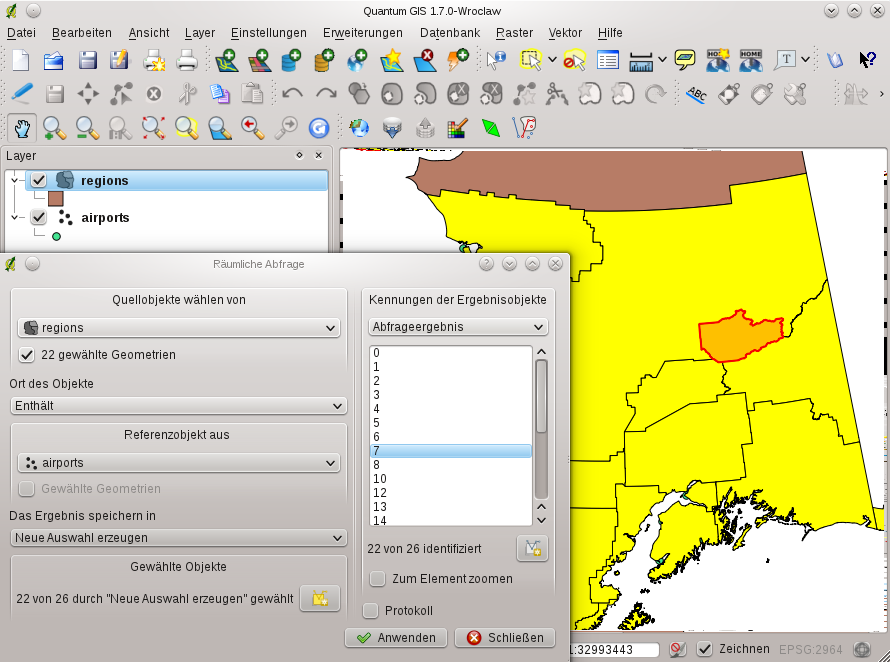
\includegraphics[clip=true, width=14cm]{spatial_query_sample}
%   \caption{Spatial Query analysis - regions contain airports \nixcaption}
   \caption{Requête Spatiale - Régions contenant des aéroports \nixcaption}
   \label{fig:spatialquerysample}
\end{figure}

\FloatBarrier
